\chapter{MATLAB}

\section{将内置函数背下来}

在MATLAB中工作时,很多操作其实都是有内置函数的,对MATLAB不熟悉就用不成,然后就“曲线救国”了,效率不高且不说,关键自己实现很费脑!这里收集一些数值计算工作中极其常用的函数。

\mintinline{Matlab}{meshgrid}

\section{如何遍历当前文件夹及其子文件夹中的全部文件?}

假设现在我们有这样一个文件夹A,它含有一些文件和子文件夹B、C、D......,这些子文件夹又包含若干层子文件夹。我们需要将这个父文件夹(A)及其子文件夹(B、C、D......)和孙文件夹中的所有文件名和其路径取出来。

如果你用的是MATLAB 2016b及更新的版本,那真的太棒了!\mintinline{Matlab}{dir()}函数已经支持遍历搜索了。尝试敲入:

\begin{minted}{Matlab}
dir_data = dir('**/*');
dir_data([dir_data.isdir]) = [];  % 去除所有.和..文件夹
\end{minted}

这将会返回一个包含文件信息的struct,现在你可以任意操作这些struct了,随意拼接路径。解放大脑,哦也!方便归方便,但是,一来肯定有大多数人使用的是MATLAB 2016b之前的版本,二来,解放大脑意味着我失去了一次独立思考的机会。

\subsection*{思考}

对于实现方法\footnote{思路来源:\href{https://stackoverflow.com/questions/2652630/how-to-get-all-files-under-a-specific-directory-in-matlab}{How to get all files under a specific directory in MATLAB?}},多层次的遍历,我第一时间想到的是递归。然后就是数据的存储了,\mintinline{Matlab}{dir()}函数返回的是一个struct,这个数据结构储存有文件的信息,我们要充分利用这个数据结构。所以现在思路是,写一个递归函数,这个函数返回包含所有文件信息的struct。

这个函数应对先处理父文件夹,获取文件和子文件夹,然后储存文件信息,同时去除子文件夹中的`.'和`..'这两个特殊文件夹。我们对获取的子文件夹再次调用该函数,并储存文件信息。如此,利用递归获取子子孙孙无穷尽文件夹的信息\footnote{其实这并不可能,因为递归是有栈高度限制的,调用函数压入栈,返回函数弹出栈,如果文件夹层次太深,一直压栈就会到达栈溢出警告的极限,例如Python的栈往往是100层,我想MATLAB的栈也大致如此,不会太高},最后函数返回存储有所有文件信息的struct。现在,你可以对这个结构体做你想做的事情。

\subsection*{解}

MATLAB 2016b以上的版本我们可以用函数返回struct,这个数据结构包含[folder, name, date, bytes, isdir, datenum]六个字段的信息,我们可以按自己意愿使用folder和name拼接出文件的完整路径。

\inputminted[firstline=1]{Matlab}{code/matlab/get_all_file_name_R2016b_newer.m}

MATLAB 2016a及之前的版本dir struct信息并不包含folder,如果返回struct,将只有文件的[name, date, bytes, isdir, datenum]五个字段的信息,所以我们并不能根据函数返回的struct拼接出文件完整路径,\textbf{我们需要自己将路径拼接成一个cell,然后使用函数返回cell}。

\inputminted{Matlab}{code/matlab/get_all_file_name_R2016a_older.m}

\subsection*{总结}
\mintinline{Matlab}{dir()}函数遍历整个F盘共2万余文件文件大约需要1.555823s。我们实现的递归函数遍历F盘文件大约需要3.703009s。慢是慢了点,但我们成功运用了递归解决问题,不是吗?

\section{如何按自然顺序排序字符串?}

通常,我们会遇到处理一系列文件名有规律的文件的情况,比如:a1.txt、a2.txt ...... a100.txt。但是,当读取文件名到一个cell里后,我们发现文件名往往是乱序排列的,甚至当你使用\mintinline{Matlab}{sort}函数后,排序也不会改变。搜索了一下,在Mathworks File Exchange网站找到了一个自然排序的函数\footnote{\url{https://cn.mathworks.com/matlabcentral/fileexchange/34464-customizable-natural-order-sort}},感谢作者Stephen Cobeldick。效果如下:

\begin{figure}[h]
    \centering
    \begin{minipage}{0.45\textwidth}
        \centering
        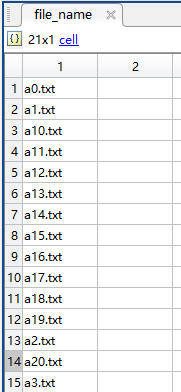
\includegraphics[height=6cm]{disordered_file_name}
        \caption{乱序的文件名}
    \end{minipage}
    \begin{minipage}{0.45\textwidth}
        \centering
        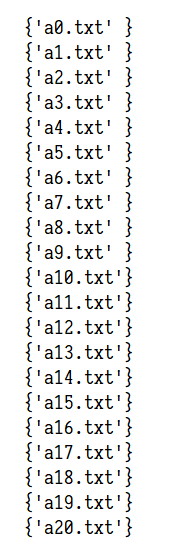
\includegraphics[height=6cm]{ordered_file_name}
        \caption{排序后自然顺序的文件名}
    \end{minipage}
\end{figure}

\section{如何隔行取数据?}

闭上眼睛,想象现在有这样一个数组\mintinline{Matlab}{[1, 2, 3, 4, 5, 6, 7, 8, 9, 10]},我们要隔一列取一个数据,或者隔两列取一个数据。得益于MATLAB的向量化编程,我们可以很方便的做到,

\begin{minted}{Matlab}
mat_a = [1, 2, 3, 4, 5, 6, 7, 8, 9, 10];
mat_b = mat_a(:, 1:2:length(mat_a));
\end{minted}

如果你用循环,那么你的代码就不优雅,另,向量化操作比循环快,大型数组优势明显。以上。

\section{如何在遍历数组的同时删除被遍历过的元素?}

闭上眼睛,想象现在有这样一个数组\mintinline{Matlab}{[1, 2, 3, 4, 5, 6, 7, 8, 9, 10]},我们需要边遍历元素边删除元素。实现方法和Python章节方法一致。

\begin{minted}{Matlab}
mat_a = [1, 2, 3, 4, 5, 6, 7, 8, 9, 10];

while ~isempty(mat_a)
    fprintf("The element being traversed is %d\n", mat_a(1));
    mat_a(1) = [];
    disp(mat_a);
end
\end{minted}

\section{再谈向量化操作}

今天又碰到一个数组操作的问题,同样,如果用一般的方法来解决,代码是很冗长的,向量化操作再次助我一臂之力。

有一个2列的数组\mintinline{Matlab}{all_data},第一列有正有负,我们称第一列为$ x $,第二列为$ y $。现在需要索引$ x>0 $时对应的$ [x, y] $为一个新的数组\mintinline{Matlab}{a}。并且需要从\mintinline{Matlab}{a}中返回$ y=\min(y) $时所对应的数组$ [x_0, y_0] $。

\begin{minted}{Matlab}
... ...
-1.44319267634370e-06 9.80637785912817e-06
-1.68967863180042e-07 9.73806551956721e-06
-6.45218837777561e-07 9.75074561060079e-06
6.28923217787410e-07 9.75037059307950e-06
1.54045071473931e-07 9.73772289244816e-06
1.42591401762642e-06 9.80510552313044e-06
... ...
\end{minted}

先谈向量化获取数组\mintinline{Matlab}{a},利用逻辑索引,保证$ x $全大于0,并取出1、2两列;然后利用\mintinline{Matlab}{find}获取$ y=\min(y) $的行索引;最后利用索引轻松找到需要的数据。可能看起来比较难理解,但是此时再在外面套文件操作的循环等循环操作是不是清晰多了。

\begin{minted}{Matlab}
a = all_data(all_data(:, 1) > 0, 1:2);

[r, ~] = find(a(:, 2) == min(a(:, 2)));
what_is_i_need = a(r, c);
\end{minted}

\begin{minted}{Matlab}
clear
clc

file_name_struct = dir('./0518*.txt');
file_name = {file_name_struct(:).name};
file_name = natsort(file_name);
what_is_i_need = [];

for file_num = 1:length(file_name)
    all_data = load(file_name{file_num});
    a = all_data(all_data(:, 1) > 0, 1:2);
    
    [r, ~] = find(a(:, 2) == min(a(:, 2)));  % 
    what_is_i_need = [what_is_i_need; a(r, 1), a(r, 2)];
end

plot(what_is_i_need(:,2))
\end{minted}

再来记录一个问题:循环操作里面有一个的2列数组\mintinline{Matlab}{all_data},每次循环取第一列中与0.5最接近的数据和对应的列,所以该数组大小会不断变,设其维度为$ n\times 2 $。如果$ n<2 $,我们将数据置为0并保存到一个新数组里面去;如果$ n>=2 $,保存其最小值和最大值到新数组里面去。同样,利用向量化操作最大程度减少代码量。

\begin{minted}{Matlab}
pos = [];
for i = 1:length(time)
    % [x, phi]
    all_data = load(strcat(mph_file, '\', num2str(i), '.txt'));
    all_data = all_data(abs(all_data(:, 2)-0.5) < 0.01, :);
    [r, c] = size(all_data);
    if r == 0 || r == 1
        x_min = 0;
        x_max = 0;
        phi = 0;
        pos = [pos; time(i), x_min, phi; time(i), x_max, phi];
    else
        x_min = all_data(all_data(:, 1) == min(all_data(:, 1)));
        x_max = all_data(all_data(:, 1) == max(all_data(:, 1)));
        [r, ~] = find(all_data == x_min);
        phi_min = all_data(r, 2);
        [r, ~] = find(all_data == x_max);
        phi_max = all_data(r, 2);
        pos = [pos; time(i), x_min, phi_min; time(i), x_max, phi_max];
    end
end
\end{minted}

\section{文件读取}

\mintinline{Matlab}{csvread}适合读取纯Comma-Separated Values文件,\mintinline{Matlab}{load}适合读取带注释的Comma-Separated Values文件(示例如下),其在读取过程中会自动忽略csv文件的注释。

\begin{minted}{Matlab}
% x                       y                        IsoLevel
-1.348651530446577E-5     1.798983884698175E-5     0.5
-1.4987361701783775E-5    2.4219367655756994E-5    0.5
-1.494145158530118E-5     2.3443649068772022E-5    0.5
... ...
\end{minted}

\section{如何将两个维度不一致的矩阵串联起来?}

现有矩阵\mintinline{Matlab}{a = [1]}和矩阵\mintinline{Matlab}{b = b = [5; 9; 4; 4]},将其横向拼接成一个矩阵\mintinline{Matlab}{c},

\begin{minted}{Matlab}
c = [1, 5;
    1, 9;
    1, 4;
    1, 4]
\end{minted}

思路很简单,因为\mintinline{Matlab}{a}的维度不够,所以将其扩维,然后拼接。

\begin{minted}{Matlab}
a = [1];
b = [5; 9; 4; 4];
[r, ~] = size(b);
c = [repmat(a, r, 1), b];
\end{minted}

\section{颜色的处理}

Hex是一种常用的十六进制颜色码,MATLAB并不能识别,从MathWorks File Exchange找了一个\mintinline{Matlab}{rgb2hex and hex2rgb}的函数\footnote{\url{https://ww2.mathworks.cn/matlabcentral/fileexchange/46289-rgb2hex-and-hex2rgb}},另,MathWorks File Exchange真特么是个宝库,缺什么找什么,一找一个准。

有时候需要将\mintinline{Matlab}{double}类型的矩阵转换成rgb色值的三维矩阵,没有MATLAB内置函数能做到,在MathWorks File Exchange上找了个\mintinline{Matlab}{double2rgb}函数\footnote{\url{https://www.mathworks.com/matlabcentral/fileexchange/30264-double2rgb}}可以很方便的做到这一点。

\section{谈谈MATLAB中的图形对象}

可视化是一项很费时费力的工作,MATLAB可视化成本更高,由于参数混杂,很难进行快速调整。我脑子不好使,先记录一下MATLAB基本图像元素的构成,更详细介绍请查阅MATLAB帮助文档\footnote{\url{https://ww2.mathworks.cn/help/matlab/graphics-objects.html}}。

\subsection{图形对象}

MATLAB的图形系统中常用的对象分为:顶层对象(Root,Figure,Axes等)、图表对象(如Bar,Contour,Surface,Line等),插图对象(如Colorbar,Legend),注释对象(如Arrow,TextBox等)和原始对象,函数对象,组对象,标尺对象等几种不常用对象。

\begin{figure}
    \centering
    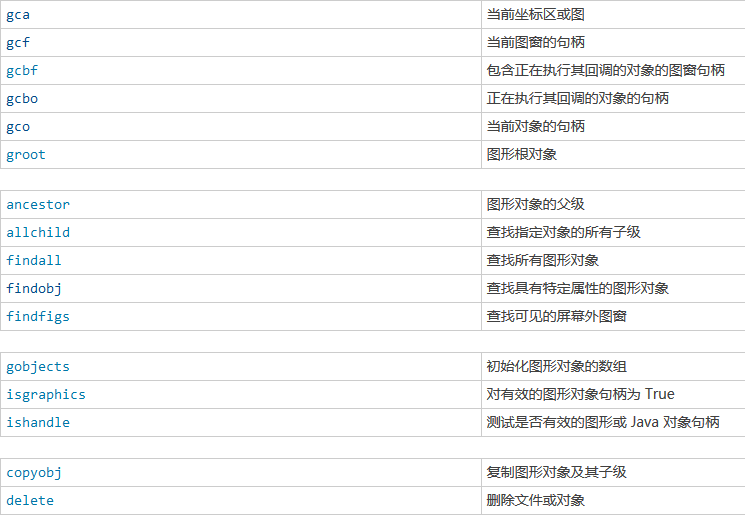
\includegraphics[height=8cm]{g_o_identification}
    \caption{MATLAB中的图形对象的标识}
    \label{g_o_identification}
\end{figure}

\begin{figure}
    \centering
    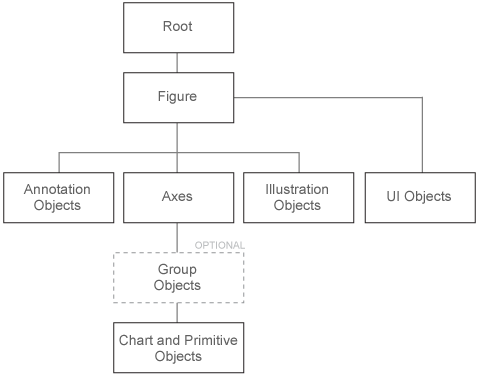
\includegraphics[height=8cm]{graphics_objects}
    \caption{MATLAB中的图形对象}
\end{figure}

我们重点关注两类对象,顶层对象\mintinline{Matlab}{Root, Figure, Axes}和插图对象\mintinline{Matlab}{Colorbar, Legend}。图形对象相关的函数如\autoref{g_o_identification}所示,用于查找、复制和删除图形对象。这些操作推荐使用面向对象编程的方式进行,代码风格如下。

\begin{minted}{Matlab}
r = groot;
fig = figure;
ax = gca;
c = colorbar;
lgd = legend('a','b','c');
\end{minted}

\mintinline{Matlab}{figure}控制图窗窗口的外观和行为,\mintinline{Matlab}{axes}控制绘图区域外观和行为的对象,图表对象(如Bar,Line等)才控制展示数据的图形的外观和行为,这几个关系一定要拎得清。如,你要修改图形窗口的大小和位置,那就改figure对象的属性;如果你要修改坐标轴的线条或者坐标轴标签,就修改axes的属性;最后,改图形内容属性,比如plot线条的粗细,你才需要修改图表对象的属性。MATLAB图形系统的设计层级关系非常明晰,理清关系才能高效进行“码”操作(笑。

\subsection{格式和注释}

大部分调整图像格式和注释的函数都是直接修改图形对象的属性,从代码可维护性的角度来看,是没必要用这些函数来修改图形的属性的。但是有一些很奇怪的函数调整的不是图像对象的属性,比如\mintinline{Matlab}{caxis}函数用于修改colorbar的色值范围,但是colorbar对象根本没有这个属性,这就卧槽了!有必要单独列出来记一下。

格式和注释分如下几类\footnote{\url{https://ww2.mathworks.cn/help/matlab/formatting-and-annotation.html}}:标题和标签、坐标区外观、颜色图、三维场景控制。

看,是吧,大部分内容直接修改图形对象的属性就可以了,但这里面偏偏有特例,可要注意了!

\subsection{子图}

\mintinline{Matlab}{subplot}函数可以画子图,有两种调用方式,

\begin{minted}{Matlab}
subplot(m,n,p)
subplot('Position',pos)
\end{minted}

第一种方式是创建一个$ m\times n $的网格,并在第$ p $个网格上绘图;第二种方式是在指定\mintinline{Matlab}{pos}上绘图,座标属性为[left bottom width height]。可以通过查阅图像对象来获取图形属性。

值得注意的是\mintinline{Matlab}{subplot}这个函数创建的是一个\mintinline{Matlab}{axes}对象,所有\mintinline{Matlab}{axes}对象可修改的属性对\mintinline{Matlab}{subplot}都起作用,哦也。

\subsection{最佳实践}

用一个图像对象的关键是搞清楚这个对象属于图像系统中的哪一类主要对象,然后去阅读该类对象的文档,切记,阅读帮助文档是最有效的解决方案。

新版本MATLAB推荐使用调用对象的方式修改图形对象属性,老版本用\mintinline{Matlab}{get, set}函数分别查阅和修改对象属性,或者使用参数传递的方法修改图形对象的属性,没有调用对象的方式优雅。下面的代码展示两种方式的区别。

\begin{minted}{Matlab}
p = plot(1:10);
p.Color = 'r';
set(p, 'Color', 'red');
\end{minted}

绘图最佳实践的代码风格如下所示,依次建立figure,axes和图表对象(如Bar,Line等),然后使用面向对象编程的方式修改其属性,有些图形属性有多层,此时切勿烦躁,及时使用\mintinline{Matlab}{get()}函数查阅对象属性。坚持使用面向对象编程,代码风格会更加清晰,不宜混乱。实际上,传参和set这两种方式最大的劣势就是不能自动补全,而且写字符串很别扭。

\begin{minted}{Matlab}
fig = figure;
ax = axes;
fig_bar = bar(cate, [all_data{:, 2}]);
ax.YLabel.String = 'Variance';
\end{minted}

\subsection{谈一谈colorbar}

colorbar这个对象属于插图对象,要修改的属性常常是位置,阅读官方文档吧\footnote{\url{https://ww2.mathworks.cn/help/matlab/ref/matlab.graphics.illustration.colorbar-properties.html}}!

怎样用代码修改colorbar的颜色和色值范围呢?这个问题困扰了我很久,一直觉得就是一行代码的事,果然不错,见官方文档\footnote{\url{https://ww2.mathworks.cn/help/matlab/ref/caxis.html}}!

\mintinline{Matlab}{caxis(target, [min max])}函数接受两个对象,目标对象可以是一个axes或者figure对象。

\begin{minted}{Matlab}
caxis(ax, [1, 100])  % 修改 ax 对象的色值范围为 1 - 100
\end{minted}

\section{函数!函数!}

这里收集几个关于函数的最佳实践,首先是函数的返回值问题。很多时候,MATLAB函数的返回值不止一个,通常让变量一一返回,在外部使用变量一一接收。最佳做法是将需要返回的变量装入\mintinline{Matlab}{struct}中,这样在外部仅使用一个变量就能接收所有返回值。

\section{如何在矩阵中插入一行/一列}

看了一圈,只能通过拼接矩阵来实现,并且MATLAB自己没有这样的函数。自己写了一个。

\begin{minted}{Matlab}
% 按行插入
function mat = row_insert(mat_row, pos, mat_add)
[~, c_row] = size(mat_row);
[~, c_add] = size(mat_add);
if c_row == c_add
    mat = [mat_row(1:pos-1, :); mat_add; mat_row(pos:end, :)];
else
    error('要插入的矩阵列要与原始矩阵一致')
end
end

% 按列插入
function mat = col_insert(mat_row, pos, mat_add)
[r_row, ~] = size(mat_row);
[r_add, ~] = size(mat_add);
if r_row == r_add
    mat = [mat_row(:, 1:pos-1), mat_add, mat_row(:, pos:end)];
else
    error('要插入的矩阵行要与原始矩阵一致')
end
end
\end{minted}

\section{图形处理}

\subsection{基本法}

\subsection{图形插值}

图形插值就是让模糊的图形(像素较少)变成比较清楚的图形(像素变多),稍微科学一点的说法是,图像插值就是利用已知邻近像素点的灰度值(或rgb值)来产生未知像素点的灰度值(或rgb值),以便由原始图像再生出具有更高分辨率的图像。图像处理的学问太多,涉及到的数学也比较深,这里只简单记录应用。

常见的插值算法有最近邻插值算法,双线性插值算法,三次卷积等。具体内容可以去学习一些DIP(Digital image processing)的公开课。如:

\url{http://inside.mines.edu/~whoff/courses/EENG510/lectures/}

\url{http://cs.nju.edu.cn/liyf/dip15/dip.htm}

常用的是MATLAB内置的\mintinline{Matlab}{interp2}函数,

Github上找了个现成的工具箱\footnote{\url{https://github.com/FlorentBrunet/image-interpolation-matlab}},快速实现bicubic和bilinear两种插值算法,效果很不错。

